\section{Konfigurationsmanagement}
Im Kapitel Konfigurationsmanagement wird die Organisationsstruktur und die Projektplanung des Projekts aufgezeigt.

\subsection{Beteiligte Personen/Rollen}
Die Semesterarbeit wird vom Studierenden dokumentiert, ausgeführt und getestet.\\
Der Auftraggeber ist der Dozent des Fachs System und Softwareengineering, \gutachter.

Während der Semesterarbeit wird der Studierende durch den Dozenten \gutachter begleitet, welcher diese Arbeit dann auch bewerten wird.

\subsection{Projektdokumentation}
Die Projektdokumentation ist auf dem Rechner des Studierenden abgelegt und wird in LaTEX geschrieben. Die Sicherung erfolgt auf OneDrive und wird mit GIT im Ordner 'docs' verwaltet. 

\subsection{Projektdaten (Code)}
Die gesamte Arbeit wird, wie auch die Dokumentation, im GIT verwaltet, damit die Änderungen nachverfolgt werden können.

\subsection{Projektmethode}
Da die Semesterarbeit mit nur einer Person gemacht wird, wird dies anhand des Sequenziellen Wasserfallmodel abgewickelt. Das Wasserfallmodel erscheint als geeignet, da dieses auf eine kürzere Projektzeit sehr gut angewendet werden kann und die Anforderungen klar dokumentiert und fixiert sind.

\begin{figure}[htp]
    \begin{center}
        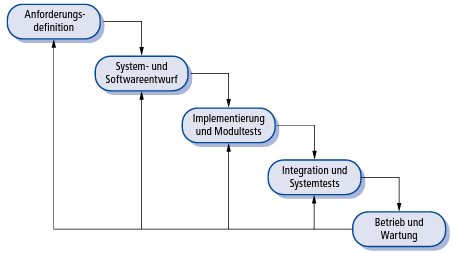
\includegraphics[width=0.5\linewidth]{content/images/wasserfallmodell.png}
        \caption{Wasserfallmodell}
        \label{fig:wasserfallmodell}
      \end{center}
\end{figure}

\newpage

\subsection{Phasen}
Wie in der \fref{fig:wasserfallmodell} zu sehen ist, besteht das Modell grundsätzlich aus den 5 Phasen.
  \begin{itemize}
      \item Analyse und Definition:\\
      Die Dienstleistungen, Einschränkungen und Ziele des Systems werden in Zusammenarbeit mit den Systembenutzern aufgestellt. Dann werden sie detaillierter  definiert und dienen so als Systemspezifikationen. 
      \item System- und Softwareentwurf:\\  Der Systementwurfsprozess weist die Anforderungen entweder Hard- oder Softwaresystemen zu. So wird eine übergeordnete Systemarchitektur festgelegt. Beim Softwareentwurf geht es um das Erkennen und Beschreiben der grundlegenden abstrakten Softwaresysteme und ihrer Beziehungen zueinander. 
      \item Implementierung und Modultests:\\  In dieser Phase wird der Softwareentwurf durch eine Menge von Programmen oder Programmeinheiten umgesetzt. Das Testen der Module stellt sicher, dass je de Einheit ihre Spezifikation erfüllt.
      \item Integration und Systemtest:\\  Die einzelnen Programmeinheiten oder Programme werden integriert und als Ganzes getestet, um sicherzustellen, dass die Softwareanforderungen erfüllt werden. Nach den Tests wird das Softwaresystem an den Kunden ausgeliefert.
      \item Betrieb und Wartung:\\ Normalerweise ist dies die längste Phase innerhalb des Lebenszyklus. Das System wird installiert und zum Gebrauch freigegeben. Zur Wartung gehören das Korrigieren von Fehlern,  die in den früheren Phasen nicht entdeckt wurden, die Verbesserung der Implementierung von Systemeinheiten und die Verbesserung des Systems, falls neue Anforderungen aufgedeckt werden
  \end{itemize}

Für die Semesterarbeit sind vor allem die Phasen 1-4 von zentraler Bedeutung.

\subsection{Planung der Phasen}

Die Detailplanung wird im DevOps mittels des dort verfügbaren Planungssystem, dem ''Delivery Plans'', erstellt und verwaltet. So können die noch zu erledigenden Arbeiten als Issue erfasst werden und sind dann in der entsprechenden Phase sichtbar.\\
Die vier Phasen werden hier in der Monatsansicht abgebildet. Die Milestones sind entsprechenden den bekannten Daten markiert.

\vspace*{3mm}

\begin{figure}[htp]
    \begin{center}
        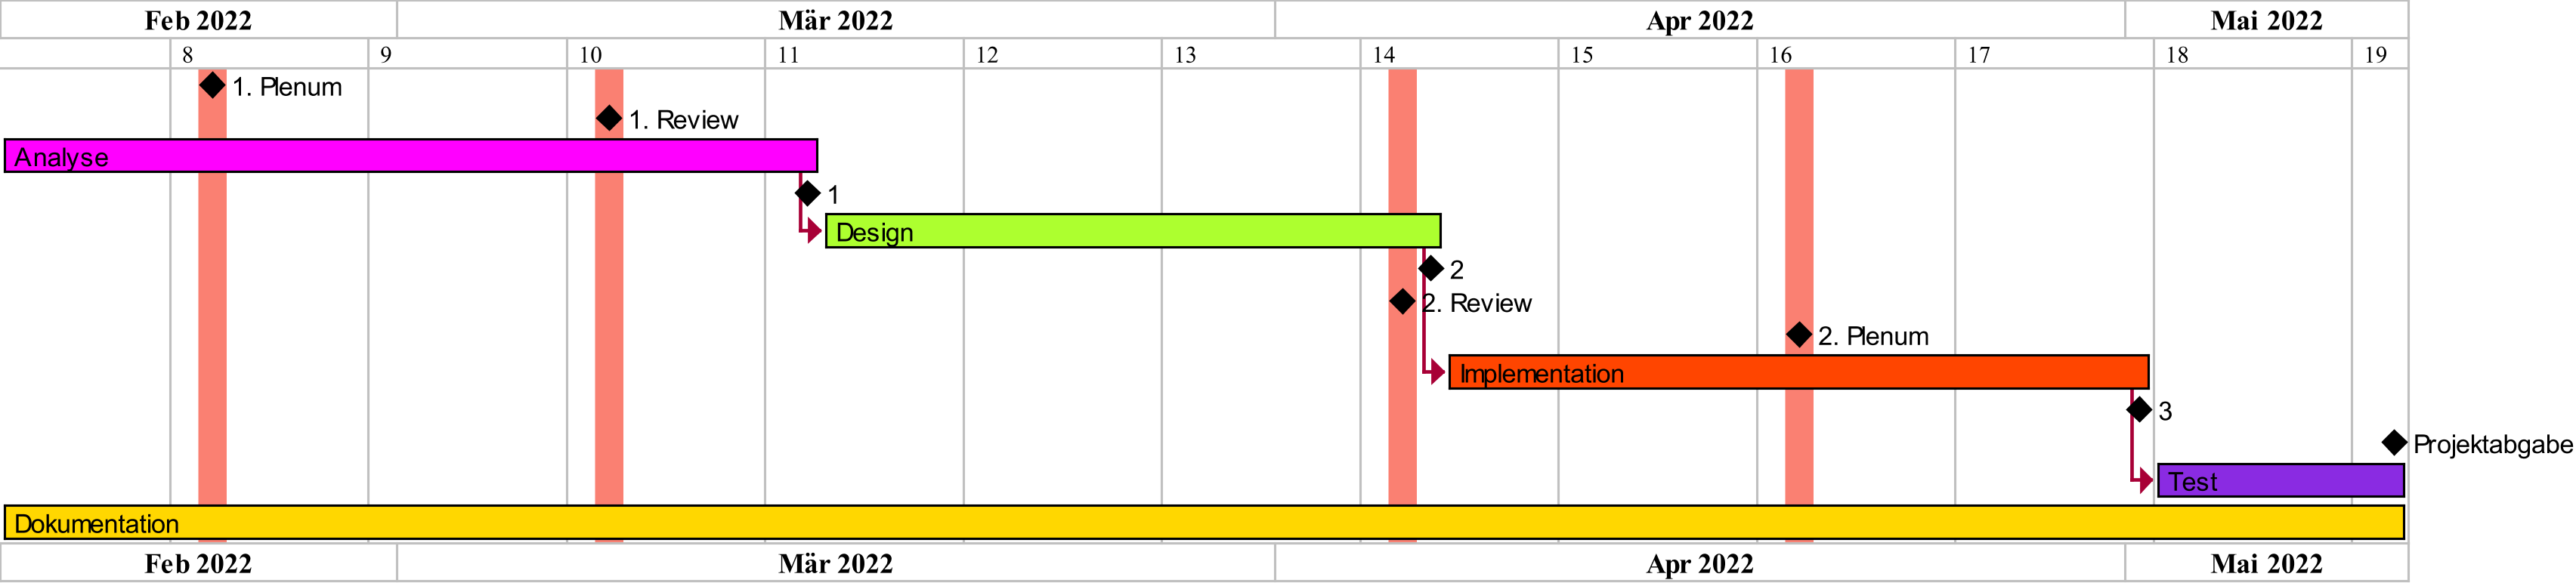
\includegraphics[width=1\linewidth]{content/diagrams/out/planning/planning.png}
        \caption{Planung}
      \end{center}
\end{figure}


